\chapter{实验结果与分析}

\section{实验设置}
实验分别考察完整系统的运行成本、三项主要优化、部署改动和功能正确性。参数来源见第2章；身份和消息采用规范字节编码，正常密码操作使用操作系统随机源。不同实验的环境与重复方式集中列于表~\ref{tab:environments}。

\begin{table}[H]
\centering\small
\caption{主要实验环境与重复方式}
\label{tab:environments}
\begin{tabularx}{\textwidth}{@{}p{.18\textwidth}Xp{.29\textwidth}@{}}
\toprule
\rowcolor{black!8} 实验 & 环境 & 输入与重复 \\
\midrule
A/B完整流程 & i9-14900HX，WSL2，Sage 10.7／Python 3.12.13，OMP 4、BLAS 1 & 身份各64 B，消息32 B；每组独立建立3套系统，每套3对重复加解密 \\
Sageloli采样 & Ultra 7 255HX，WSL2，Python 3.13.15，OMP与BLAS均4 & PARAM-I、II各建立1套；身份21 B、消息33 B及后续消息 \\
SRGG编码 & Ultra 7 255HX，WSL2，Python 3.13.15，OMP与BLAS均1 & 每档3套系统；同对象交替测量两种编码各5次 \\
Lai完整组合 & Ultra 9 275HX，WSL2，Sage 10.9／Python 3.13.14，OMP与BLAS均1 & 身份各64 B，消息32 B；C组合1次，解密进程存在并发 \\
接收会话 & 与A/B主实验的机器及运行时相同 & 1套系统；原解密2次，准备1次，会话解密3次 \\
部署位置 & Ultra 9 275HX，WSL2，Python 3.13.14，OMP 4、BLAS 1 & 相同3套状态；每种位置各30次完整加密、解密 \\
\bottomrule
\end{tabularx}
\end{table}

完整流程计时包含组合编码、对象检查和原语调用。首次解密包含叶钥生成；恢复实验另起进程加载已有对象。表中重复测量描述固定密钥下的运行波动，独立建立系统的数量单独列出。下文时间通常保留3位有效数字；B、KiB、MiB分别表示字节、$2^{10}$字节和$2^{20}$字节。

\section{完整系统的时间与存储成本}
\subsection{固定HIBE后的A/B对照}
A、B使用相同LATTE参数与相同输入，主要差别在IBS。表~\ref{tab:ab-times}给出完整生命周期的中位时间，图~\ref{fig:ab-times}展示重复加解密的各次测量。

\begin{table}[H]
\centering\small
\caption{A/B完整流程中位时间，单位为秒}
\label{tab:ab-times}
\begin{tabular}{@{}lrrr@{}}
\toprule
\rowcolor{black!8} 操作 & A & B & 测量次数（A/B） \\
\midrule
% BEGIN DATA ab-timings.tex
系统建立 & 1.12 & 1.6 & 3/3 \\
发送者发钥 & 0.0954 & 32.1 & 3/3 \\
接收者发钥 & 0.427 & 0.457 & 3/3 \\
首次加密 & 0.0963 & 9.14 & 3/3 \\
首次解密 & 0.284 & 0.239 & 3/3 \\
重复加密 & 0.0785 & 9.17 & 9/9 \\
重复解密 & 0.152 & 0.161 & 9/9 \\
对象恢复 & 0.845 & 0.89 & 3/3 \\
恢复后解密 & 0.154 & 0.134 & 9/9 \\
% END DATA ab-timings.tex
\bottomrule
\end{tabular}
\end{table}

两组接收者发钥和重复解密接近，额外成本主要出现在B的发送者发钥与签名生成。A、B重复加密中位数分别为78.5毫秒和9.17秒，重复解密分别为152毫秒和161毫秒。A适合作为交互演示基线；B展示原生模块格IBS在同一完整协议中的运行特点。

\begin{figure}[H]
\centering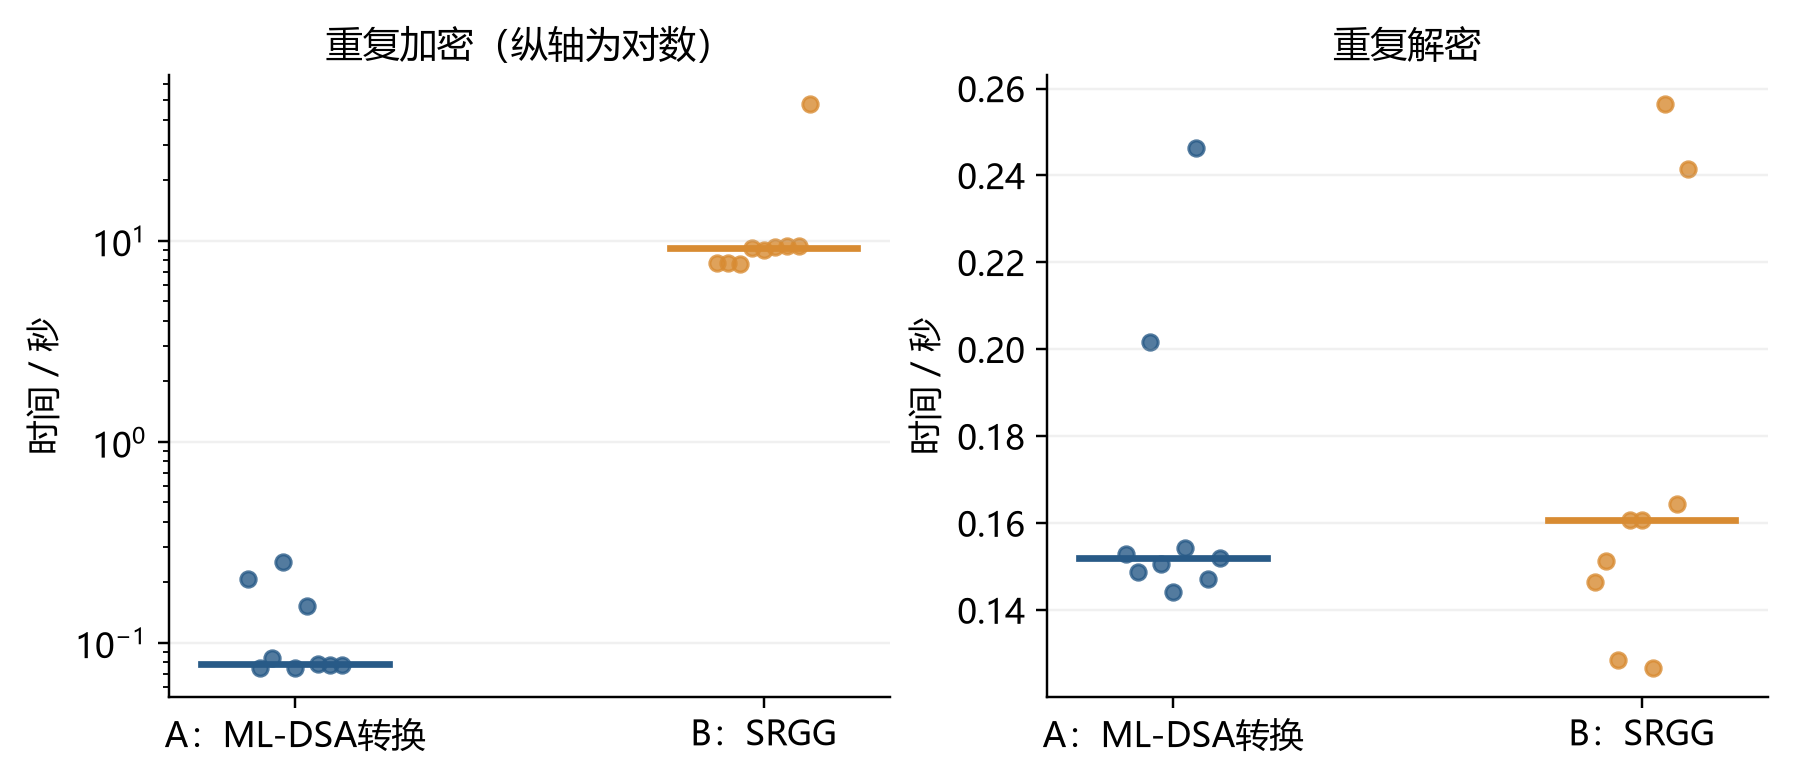
\includegraphics[width=.98\textwidth]{figures/ab-times.png}
\caption{A/B重复操作的时间分布。每组3套系统、每套3次，横线为中位数；加密面板使用对数纵轴}
\label{fig:ab-times}
\end{figure}

各次测量还说明只看中位数会遗漏波动。B有一次重复加密耗时约48.2秒，明显高于其中位数；A也存在较慢观测。首次解密高于重复解密，与叶钥生成有关。恢复对象后，解密回到重复操作相近的量级。

\subsection{对象尺寸与运行内存}
表~\ref{tab:ab-sizes}汇总公共对象、主状态和双方密钥的编码长度。A、B完整密文约139 KiB和146 KiB；第5.3节进一步解释其组成。

\begin{table}[H]
\centering\small
\caption{A/B对象编码长度约值与运行内存}
\label{tab:ab-sizes}
\begin{tabular}{@{}crrrrrr@{}}
\toprule
\rowcolor{black!8} 组 & 公钥 & 主状态 & 发送钥 & 接收状态 & 完整密文 & 内存/MiB \\
\midrule
% BEGIN DATA ab-sizes.tex
A & 14 & 173 & 7.86 & 125 & 139 & 460 \\
B & 46.2 & 262 & 82.4 & 125 & 146 & 485 \\
% END DATA ab-sizes.tex
\bottomrule
\end{tabular}
\begin{minipage}{.96\textwidth}\footnotesize
前五项单位为KiB。对象长度按记录范围取近似值；内存为每10毫秒采样的进程树RSS最高值，包含运行库和子进程，短时峰值可能未被采样捕获。
\end{minipage}
\end{table}

B的公钥、主状态与发送钥大于A，接收状态接近，符合两组共用HIBE而采用不同IBS的结构。编码文件大小和运行内存分别统计：紧凑密钥文件加载后仍会恢复为数学对象，运行时还需要数值库、采样工作区和子进程。

\subsection{C的主要耗时来自委派}
在C的一次32字节消息组合测试中，加密耗时99.0秒，匹配解密425秒，其中Lai委派为393秒，占约92.5\%。这说明对固定通信双方，重复生成同一身份路径的叶钥是优先优化的位置。该次数据来自Ultra 9机器，解密进程存在并发，用于分析其阶段组成。

C的传输密文约4.34 MiB，大部分来自Sageloli签名和Lai胶囊。它展示了另一类HIBE与环IBS在论文配置下的完整组合，以及会话摊销的使用方式。下面分别分析通信量与准备成本。

\section{小消息为什么仍产生较大的密文}
\subsection{完整密文的组成}
混合加密使应用消息不再受HIBE短明文容量直接限制，但种子胶囊、IBS签名和一次性认证仍需要传输。依据现有安装运行记录与实际编码格式，可将A的一条32字节消息和C的一条空消息分解为表~\ref{tab:ciphertext-parts}。

\begin{table}[H]
\centering\small
\caption{两条已有密文的字节组成核算}
\label{tab:ciphertext-parts}
\begin{tabular}{@{}lrr@{}}
\toprule
\rowcolor{black!8} 组成部分 & A：消息32 B & C：空消息 \\
\midrule
一次性公钥 & 65,536 & 65,536 \\
一次性签名 & 32,768 & 32,768 \\
IBS签名 & 6,237 & 3,227,824 \\
HIBE胶囊 & 37,088 & 1,228,844 \\
应用消息 & 32 & 0 \\
上下文、格式、nonce与标签 & 432 & 432 \\
\midrule
合计 & 142,093 & 4,555,404 \\
\bottomrule
\end{tabular}
\begin{minipage}{.96\textwidth}\footnotesize
整包长度来自已有运行；固定字段按序列化模块核算，HIBE胶囊长度由整包扣除其他组成得到。该核算没有新增加密实验。
\end{minipage}
\end{table}

\begin{figure}[H]
\centering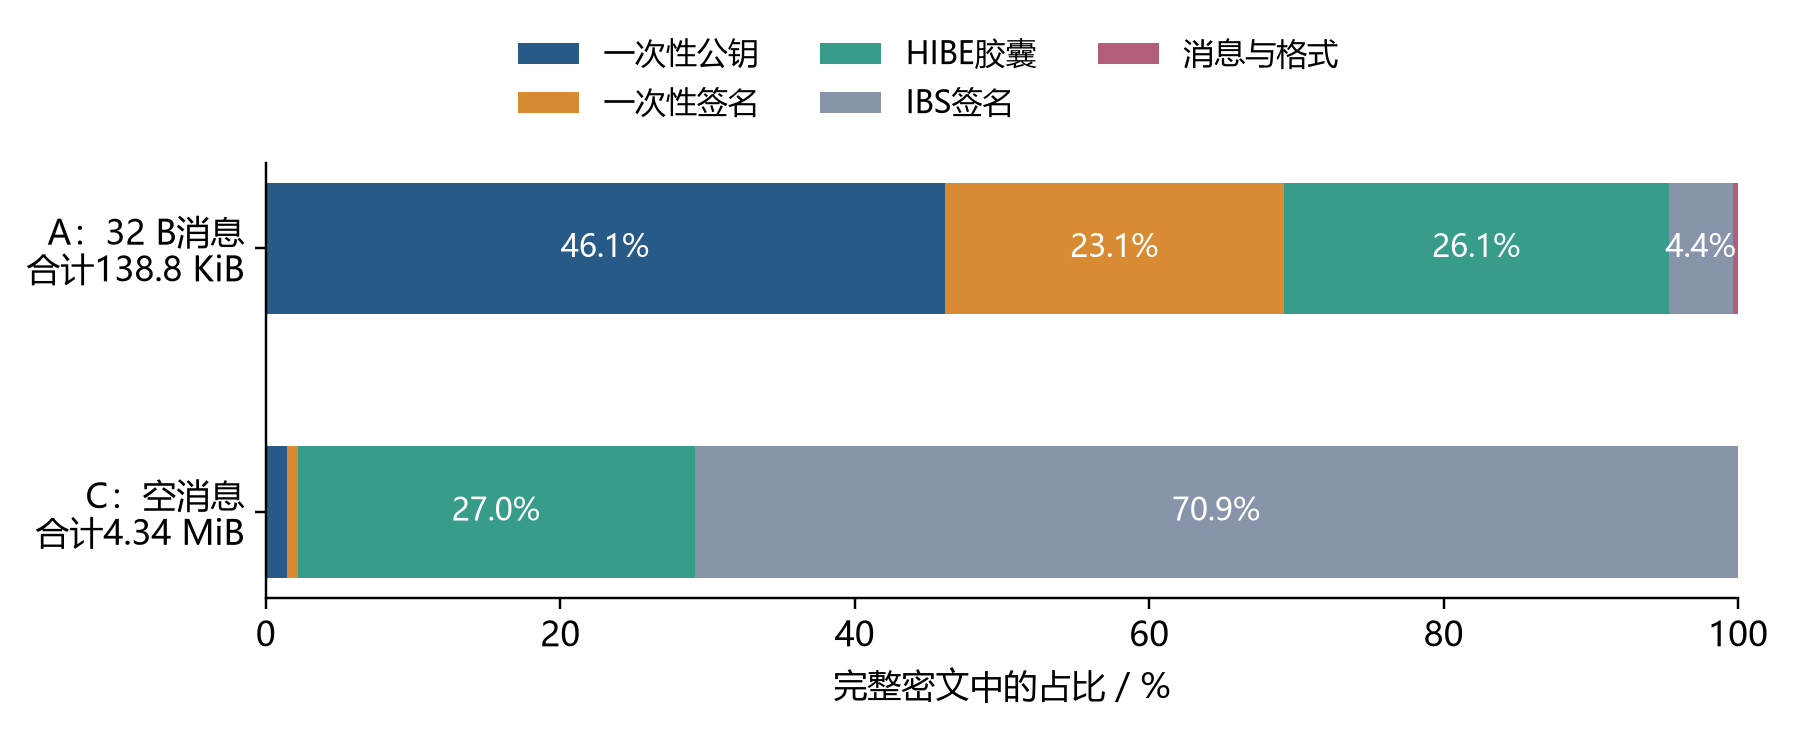
\includegraphics[width=.98\textwidth]{figures/ciphertext-parts.png}
\caption{完整密文的主要成本来源：A以一次性认证为主，C以IBS签名和HIBE胶囊为主}
\label{fig:ciphertext-parts}
\end{figure}

Lamport一次性公钥含1,024个64字节哈希像，签名含512个64字节原像，两项合计固定96 KiB，约占这条A密文的69.2\%。因此，缩短几字节应用消息几乎不会改变A的整包长度。C的IBS签名约占70.9\%，HIBE胶囊约占27.0\%；其后续通信优化应优先考察这两部分。

这也解释了SRGG签名紧凑编码与完整B密文的关系：签名字段变短会减少对称载荷，但整包还包含与A相同的一次性认证结构和LATTE胶囊。评价编码时应同时看单体对象与完整协议中的占比。

\subsection{消息长度与可用容量}
安装运行测试已完成A的0、32、1,024和59,191字节消息，B的0、32、1,024和65,364字节消息；超过应用上限1字节时，系统在生成新密文前拒绝。该批最大长度密文约为197 KiB和210 KiB。

C已完成空消息和1,024字节消息，两条密文相差1,024字节，符合固定胶囊与签名加上可变应用载荷的组成。C的3,924字节上限来自容量计算，尚缺该最大长度的加密解密记录。上述容量检查使用签名保守上界，具体签名和胶囊的编码长度仍可能随随机输出变化。

\section{三项主要优化的效果}
\subsection{结构化采样使论文规模进入实际运行}
Sageloli两个参数档均完成建立、身份发钥、两次签名和验证。表~\ref{tab:sageloli-times}给出各档一套系统的运行记录。

\begin{table}[H]
\centering\small
\caption{Sageloli结构化实现的实际运行，时间单位为秒}
\label{tab:sageloli-times}
\begin{tabular}{@{}lrrrrrr@{}}
\toprule
\rowcolor{black!8} 参数档 & 建立 & 发钥 & 首次签名 & 后续签名 & 验证 & RSS/GiB \\
\midrule
% BEGIN DATA sageloli-times.tex
PARAM-I & 4.99 & 85.1 & 9.28 & 2.02 & 0.517 & 1.36 \\
PARAM-II & 43.6 & 520 & 38.6 & 5.02 & 1.36 & 6.19 \\
% END DATA sageloli-times.tex
\bottomrule
\end{tabular}
\end{table}

PARAM-I发钥约85.1秒，记录峰值RSS约1.36 GiB；PARAM-II发钥约520秒，约6.19 GiB。首次签名明显高于第二次，与同一身份陷门下数值准备的复用相符。结构化实现的主要成果是让这些参数下的采样与验证能够实际完成。稠密矩阵的1.18 TiB是第3章按表示方式计算的存储估算，实验记录对应结构化实现。

\subsection{紧凑编码的收益集中在大整数对象}
图~\ref{fig:codec}和表~\ref{tab:codec-sizes}展示三档SRGG相同数学对象的两种编码。每档独立建立3套系统，在同一对象上交替执行两种格式的编解码。

\begin{figure}[H]
\centering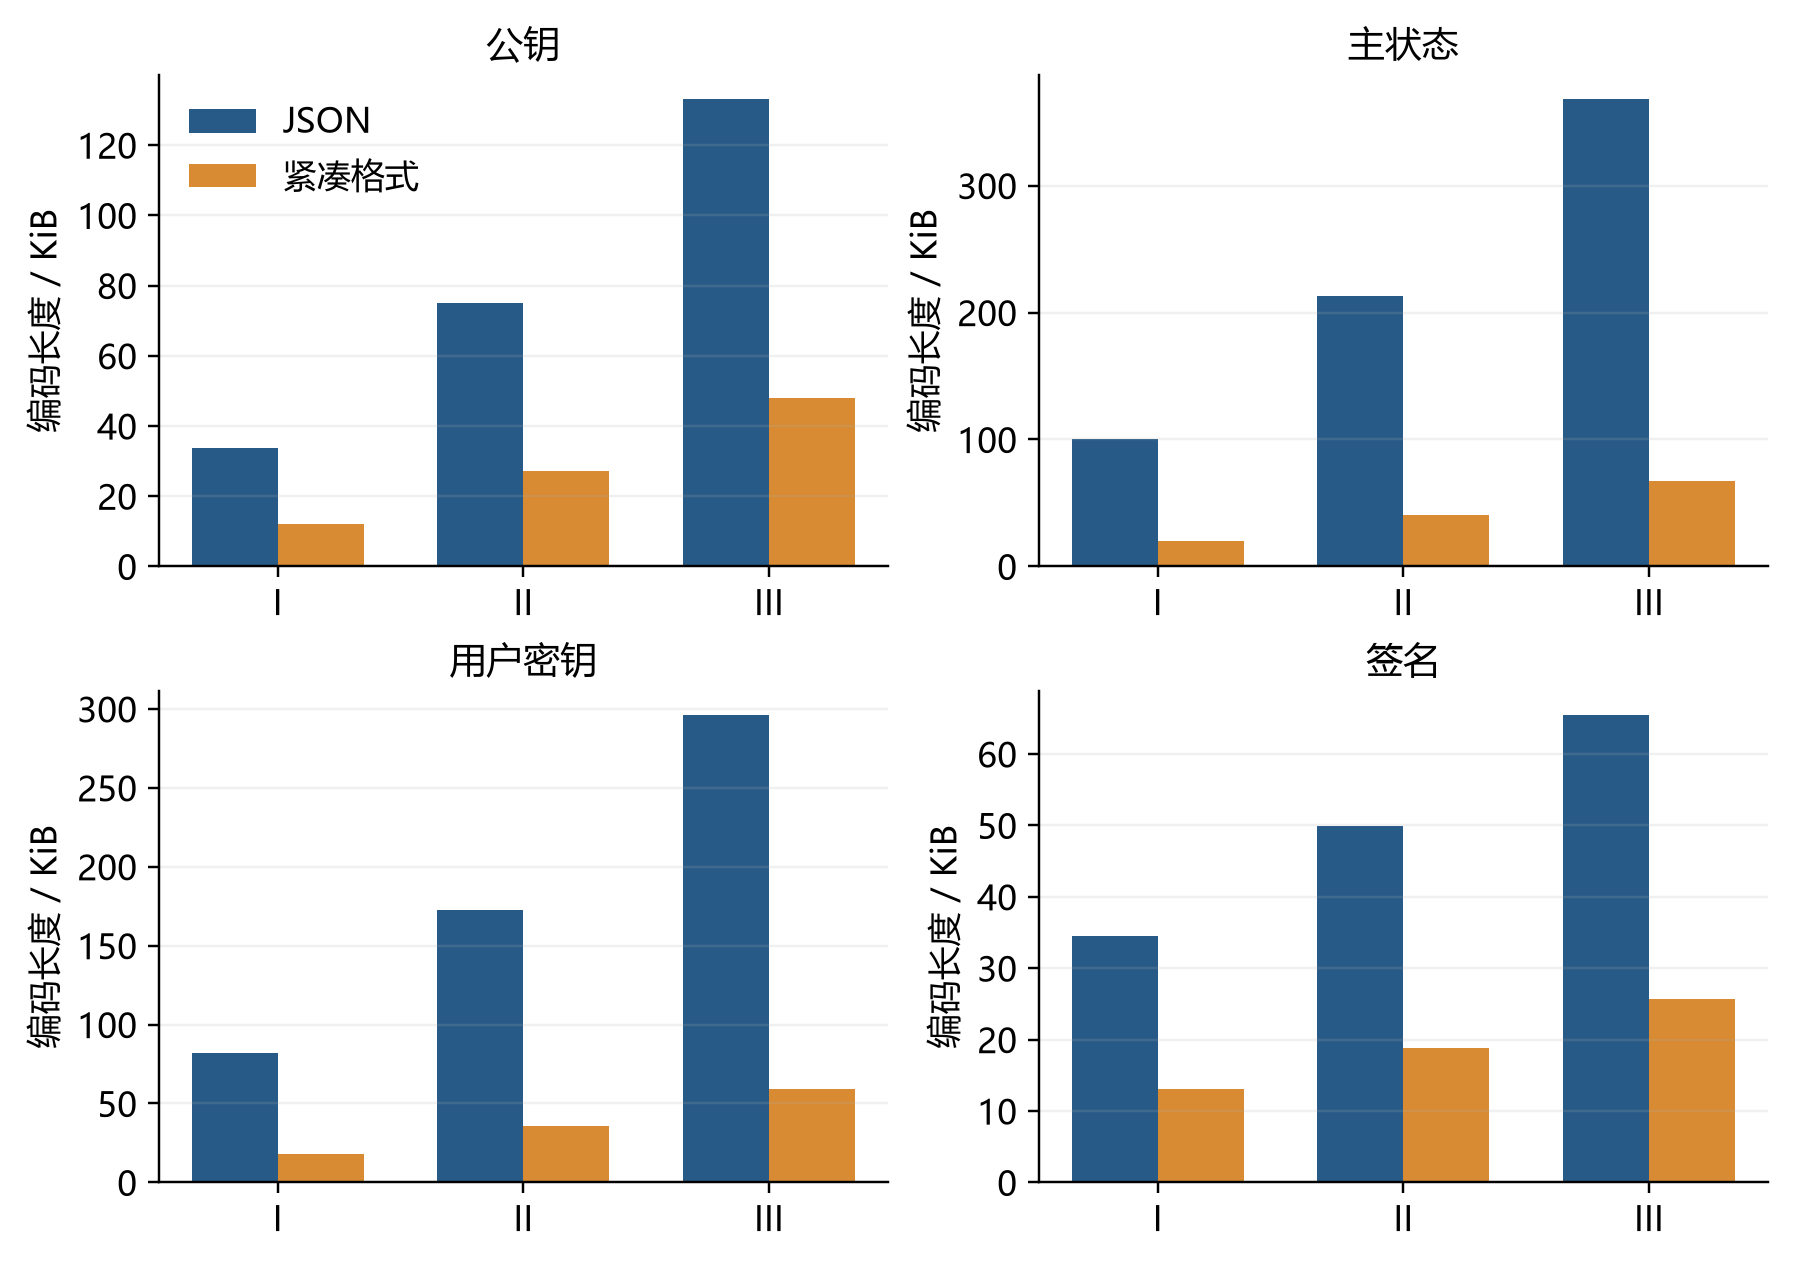
\includegraphics[width=.96\textwidth]{figures/codec.png}
\caption{SRGG三档参数的四类对象尺寸；I、II、III表示参数档}
\label{fig:codec}
\end{figure}

\begin{table}[H]
\centering\small
\caption{SRGG对象编码长度，单位为KiB}
\label{tab:codec-sizes}
\begin{tabular}{@{}lrrrr@{}}
\toprule
\rowcolor{black!8} 参数档／格式 & 公钥 & 主状态 & 用户钥 & 签名 \\
\midrule
% BEGIN DATA codec-sizes.tex
I／JSON & 33.7 & 100 & 82.2 & 34.5 \\
I／紧凑 & 12.1 & 19.8 & 17.8 & 13.1 \\
II／JSON & 75.2 & 213 & 173 & 49.9 \\
II／紧凑 & 27.1 & 40.1 & 35.6 & 18.8 \\
III／JSON & 133 & 368 & 296 & 65.5 \\
III／紧凑 & 48.1 & 67.5 & 59.5 & 25.6 \\
% END DATA codec-sizes.tex
\bottomrule
\end{tabular}
\end{table}

公钥长度缩小约2.77至2.79倍，主状态5.05至5.46倍，用户钥4.61至4.98倍，签名2.55至2.65倍。主状态包含较多小范围陷门系数，去除十进制和结构符号开销后，缩减最明显。

紧凑格式需要位打包、取值检查和规范解码。例如PARAM-I主状态的紧凑编码与解码阶段中位时间约23.1和61.3毫秒，JSON约0.974和37.3毫秒。该项优化的主要收益是对象存储与传输长度，适用于重视密钥保存和通信量的使用方式。

\subsection{接收会话把准备成本分摊到连续消息}
Lai会话实验使用一套主密钥，原路径解密2次，建立会话1次，会话内解密3次。原解密中位数为526秒，会话准备约510秒，后续解密中位数为28.6秒，额外保留叶钥编码34.7 MiB。

\begin{figure}[H]
\centering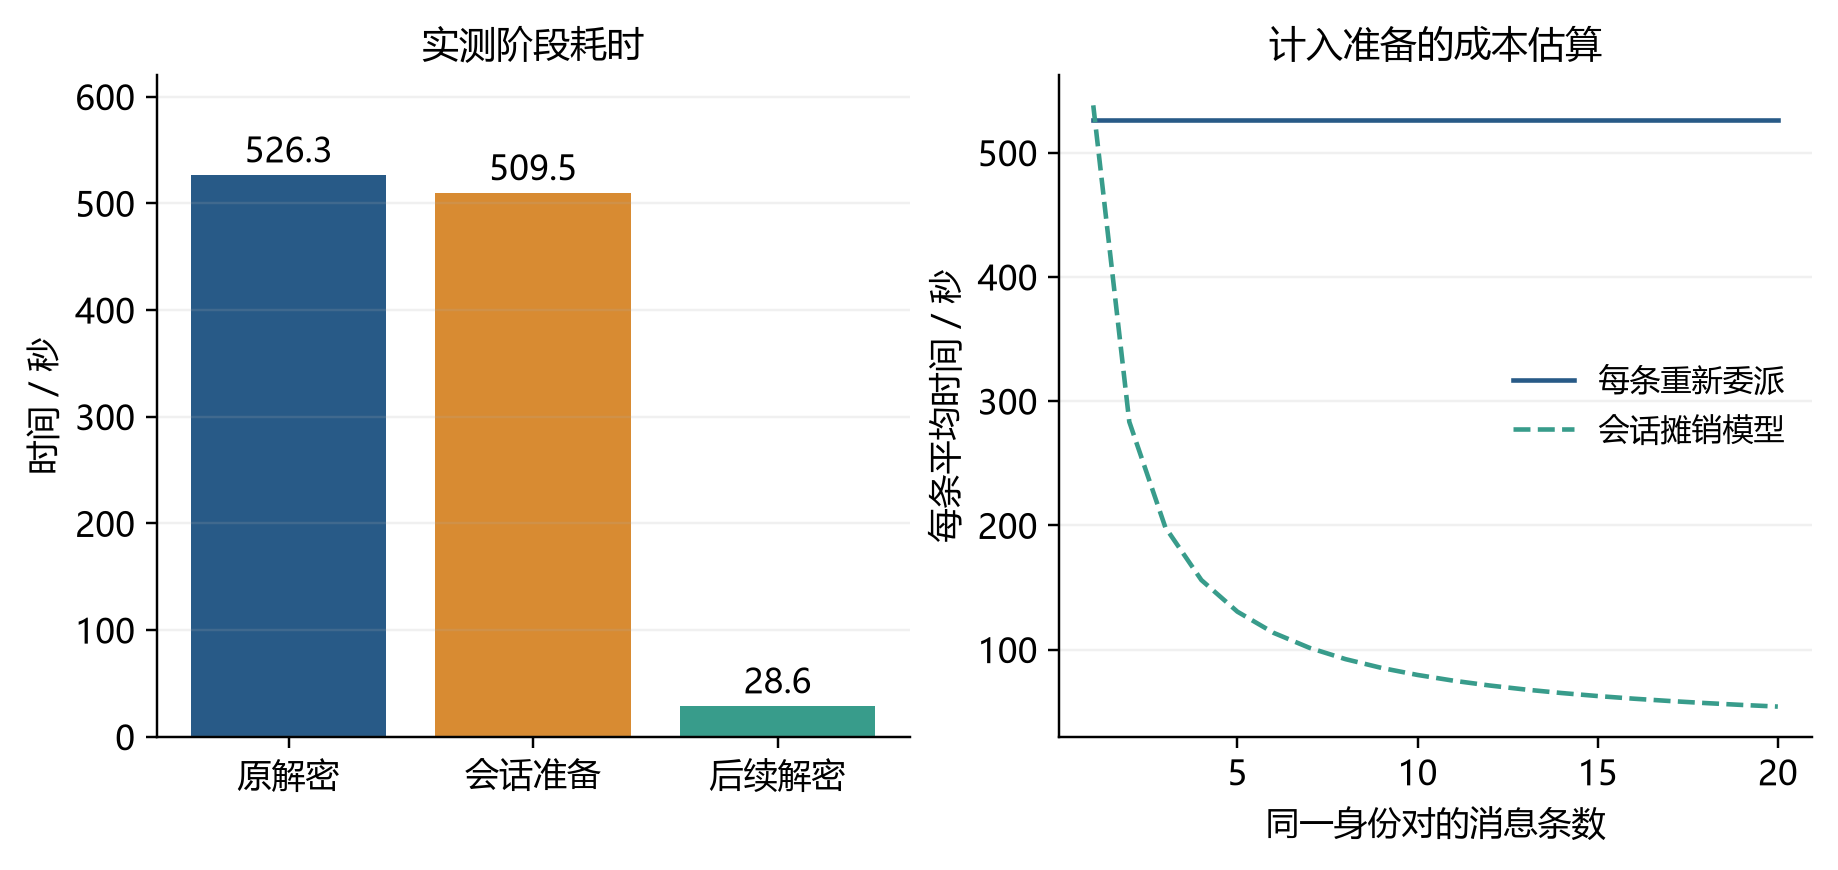
\includegraphics[width=.98\textwidth]{figures/session.png}
\caption{Lai接收会话：左图为测得阶段耗时，右图由阶段中位数代入成本公式估算}
\label{fig:session}
\end{figure}

准备完成后的单条时间约为原路径的$1/18.4$。把准备计入后，首条平均成本约538秒；按$\bar T(N)$模型，处理10条和100条消息时约为79.5秒和33.7秒。右图使用已有阶段耗时外推消息数量，未逐条执行整条曲线。

会话方法把主要委派开销移到首次使用，适合固定身份对的连续消息。短暂的一次通信仍要承担完整准备；长期会话则以额外秘密状态换取较低的后续延迟。该组样本来自一套系统，后续扩大测量可进一步观察不同主密钥下的波动。

\section{缓存与部署位置的完整流程对照}
\subsection{局部缓存对总耗时的影响}
在A、B各3套系统中，分别开启和关闭优化，以相同输入执行完整流程。A缓存机构证书的成功验证结果，原生验签调用由每条2次减少为1次，解密时间比中位数为1.086，逐套范围0.992至1.339。B复用签名数值准备，加密时间比中位数1.030，范围1.009至1.921。

这些结果说明，减少一次局部调用后，总时间仍受其余密码运算与运行波动影响。A有一套测量略微回退，B的中位收益较小。因此，系统保留缓存容量与关闭选项，主要优化结论仍以结构表示、编码和Lai会话为重点。

\subsection{同一运行时下比较文件位置}
三路部署对照固定参数、状态和原生引擎，均由同一WSL Python运行，分别使用Windows盘源码、Windows盘安装包及Linux盘同一安装包。每路完成30次完整加密和30次解密，图~\ref{fig:placement}给出中位数。

\begin{figure}[H]
\centering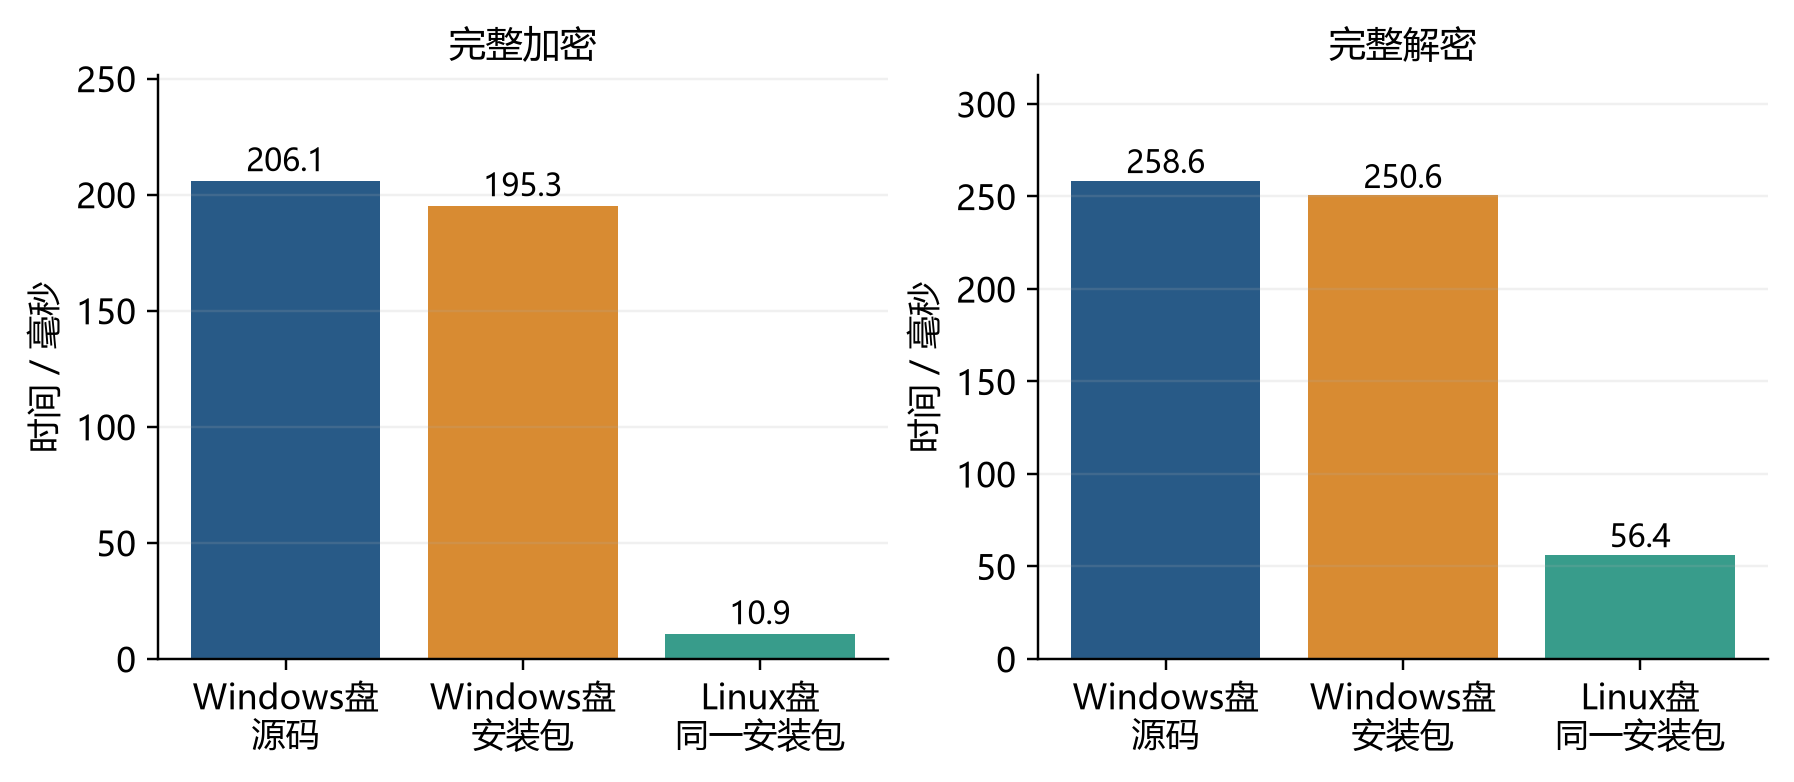
\includegraphics[width=.98\textwidth]{figures/placement.png}
\caption{文件放置位置对完整A流程的影响；三路均使用同一WSL运行时}
\label{fig:placement}
\end{figure}

Linux盘安装包相比Windows盘源码，加密与解密时间比分别约18.87和4.59；只比较同一安装包的两种位置，时间比约17.88和4.45。剖析显示，5次加密的515次文件读取在挂载目录累计约1.073秒，在Linux本地约0.011秒。文件访问是该批运行的重要成本，本机部署优先采用Linux本地目录。

\section{功能测试结果}
三组均完成双方匹配恢复和三类身份错配拒绝。表~\ref{tab:functional}汇总主要检查；另有A的随机身份与消息批次，独立建立3套系统、测试12组输入，60/60项判断符合预期。

\begin{table}[H]
\centering\small
\caption{三组完整协议的主要功能结果}
\label{tab:functional}
\begin{tabularx}{\textwidth}{@{}Xccc@{}}
\toprule
\rowcolor{black!8} 检查情况 & A & B & C \\
\midrule
双方身份匹配 & 恢复原文 & 恢复原文 & 恢复原文 \\
仅接收身份不匹配 & 拒绝 & 拒绝 & 拒绝 \\
仅期望发送身份不匹配 & 拒绝 & 拒绝 & 拒绝 \\
双方身份都不匹配 & 拒绝 & 拒绝 & 拒绝 \\
密文字节修改、截断、追加或重复字段 & 拒绝 & 拒绝 & 拒绝 \\
外层认证有效、内部签名无效 & 拒绝 & 拒绝 & 拒绝 \\
新进程加载对象后解密 & 成功 & 成功 & 成功 \\
\bottomrule
\end{tabularx}
\end{table}
